\documentclass[11pt]{article}
\usepackage{graphicx}
\usepackage{cite}
\def\BibTeX{{\rm B\kern-.05em{\sc i\kern-.025em b}\kern-.08em
    T\kern-.1667em\lower.7ex\hbox{E}\kern-.125emX}}
\usepackage{url}
    \makeatletter
    \g@addto@macro{\UrlBreaks}{\UrlOrds}
    \makeatother
\usepackage{appendix}
\usepackage[version=3]{mhchem}
\usepackage{amsmath}
\usepackage{booktabs}
\renewcommand{\arraystretch}{1.2}
\usepackage{amssymb}
\usepackage{float}
\usepackage{commath}
\usepackage{siunitx}
\usepackage{multirow}
\usepackage[a4paper,margin=20mm]{geometry}
\setlength{\parskip}{\baselineskip}%
\setlength{\parindent}{0pt}%
\sisetup{detect-all}
\begin{document}
\title{\textbf{UCL Mechanical Engineering}\\MECH0015\\ Failure Analysis Case Study\\
of a Car Suspension Spring}
\author{Group 10}
\maketitle
\begin{table}[H]
	\centering
	\begin{tabular}{@{}llll@{}}
      	\toprule
		Student name & Degree course \& year & Personal tutor's name & Contribution\\
		\midrule
		Kofoworolaoluwa Babalola & MEng Mechanical Engineering  & Dr Midhat Talibi&14.29\%\\
		& Year 2 & & \\
		Ariff Mohd Nazalan & MEng Mechanical Engineering & Dr Yuanchang Liu & 14.29\%\\
		& Year 2 & & \\
		Hasha Dar & MEng Mechanical Engineering  & Dr Andrea Ducci & 14.29\%\\ 
		& Year 2 & & \\
		Clara Hyeonji Kim & MEng Mechanical Engineering & Dr Paul Fromme & 14.29\%\\
		& Year 2 & & \\
		Lim Chern Yao & MEng Mechanical Engineering & Dr Suwan Jayasinghe & 14.29\%\\
		& Year 2 & & \\
		Xueqing Lu (Sherry) & MEng Mechanical Engineering  & Dr Will Newton & 14.29\%\\
		& Year 2 & & \\
		Ryan Surayan & MEng Mechanical Engineering  & Dr Mehran Moazen & 14.29\%\\
		& Year 2 & & \\
		\midrule
		\multicolumn{4}{c}{\textbf{I acknowledge that this is a fair estimation of my contribution.}} \\
      	\bottomrule
	\end{tabular}
\end{table} 
\tableofcontents
\listoffigures
\newpage
\section{Introduction and background}
\subsection{What is a suspension system?}
A suspension spring is part of a car’s suspension system. The suspension system consists of several parts such as tires, linkages, dampers and springs that are collectively used to support the car and maintain tire contact on the irregular surface of a road. This allows the user to turn corners and go over bumps safely whilst ensuring a comfortable ride. These components are situated on both ends of the car near the wheel axle. Without a suspension system, proper road handling and drive quality of the car would be virtually non-existent.   
\subsection{Springs}
Modern car suspension spring systems utilise 4 different designs – coil springs, leaf springs, air springs and torsion bars. This report focuses on a coil spring which is simply a steel rod that has been coiled around an axis. It is designed to stretch and compress due to vertical movement of the wheels and absorb shock as the car drives over bumps and irregularities on the road. It does so by converting kinetic energy into elastic potential energy which will be dissipated when the spring returns to its equilibrium position.
\begin{figure}[H]
    \centering
    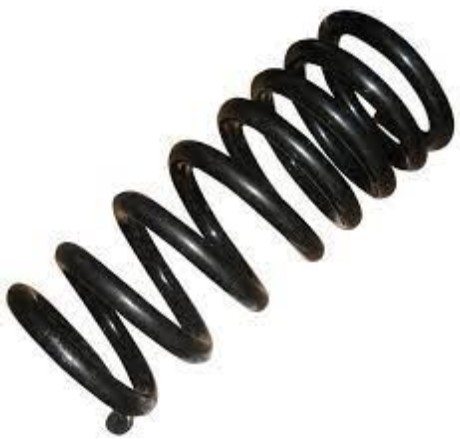
\includegraphics[height = 7cm]{./img/spring1.png}
    \caption{A typical spring.}
    \label{fig:spring1}
\end{figure}
\subsection{Dampers}
Whilst coil springs are excellent at absorbing shock, they are not as good at dissipating the stored energy which is where dampers are used. A damper is a shock absorber that controls and reduces unwanted spring motion through dampening. A damper consists of a piston that moves inside a sealed, oil-filled chamber that has special valves which only allow a slow transfer of fluid between the pressure tube and the reserve tube. Dampening works by converting the kinetic energy from the suspension movement into thermal energy as the piston forces oil to move from one tube to another at a slow rate. The heat energy will then naturally dissipate through the oil or hydraulic fluid. 
\begin{figure}[H]
    \centering
    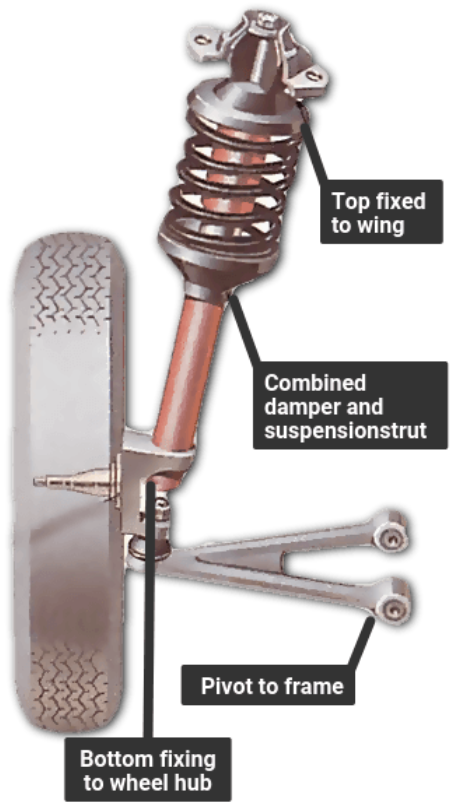
\includegraphics[height = 11cm]{./img/damper1.png}
    \caption{Diagram of a damper used in a suspension system.}
    \label{fig:damper1}
\end{figure}
\subsection{Function}
The coil spring is a mechanical device used in a car suspension system to absorb shock from the vertical movements of a car. When the spring compress and is in compression, it has converted incoming kinetic energy into elastic potential energy, which will then be released as the spring expands and returns to its original shape. As time goes by, the spring will lose elasticity with general usage and fatigue, potentially causing failure which will be discussed further in this report.  
\newpage
\section{Design analysis}
\subsection{Simulation setup}
To further investigate the loads that the suspension coil spring experiences while under operation, a CAD model was created on Fusion 360, and a Finite Element Analysis (FEA) was conducted. The purpose of this simulation is to understand whether the failure is caused due to the loadings experienced by the coil while operated.  

A suspension coil with the exact dimensions as the case study is produced and loads imitating average conditions that a sedan car experiences were placed on the model. 
\begin{figure}[H]
    \centering
    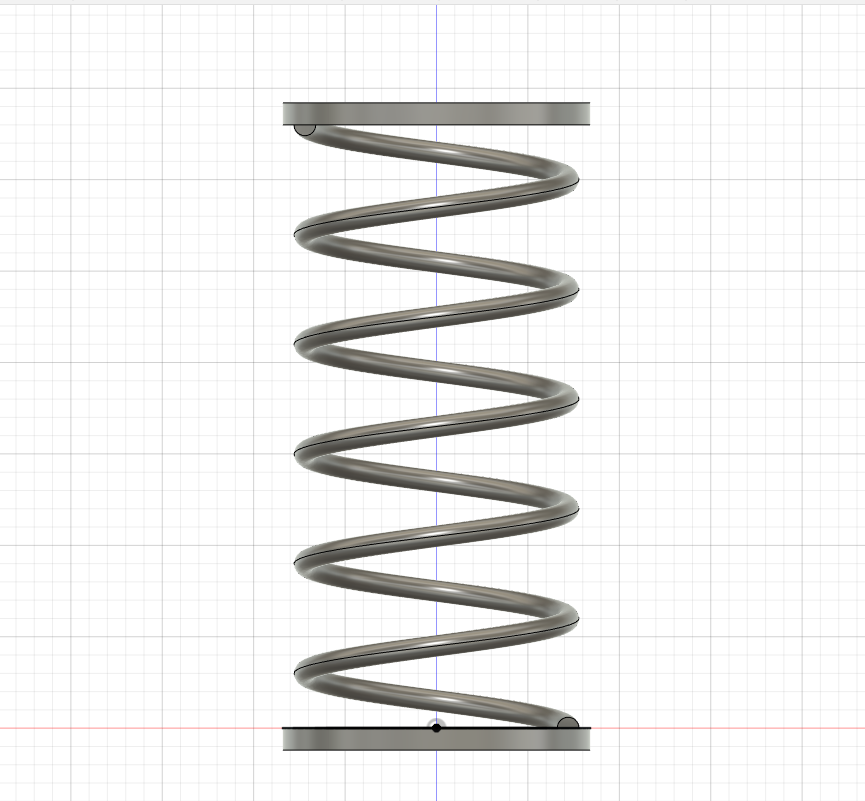
\includegraphics[height = 10cm]{./img/springmodel.png}
    \caption{Screenshot from Fusion 360, showing CAD model of a spring, with compression plates.}
    \label{fig:cad1}
\end{figure}
\begin{table}[H]
    \centering
    \begin{tabular}{@{}ll@{}}
        \toprule
        Wire diameter & \SI{6}{\milli\meter}\\
		Outer diameter & \SI{144}{\milli\meter}\\
		Length & \SI{330}{\milli\meter}\\
		Number of coils & 5.5\\
        \bottomrule
    \end{tabular}
	\caption{Table outlining dimensions of CAD model spring.}
\end{table}
\begin{figure}[H]
    \centering
    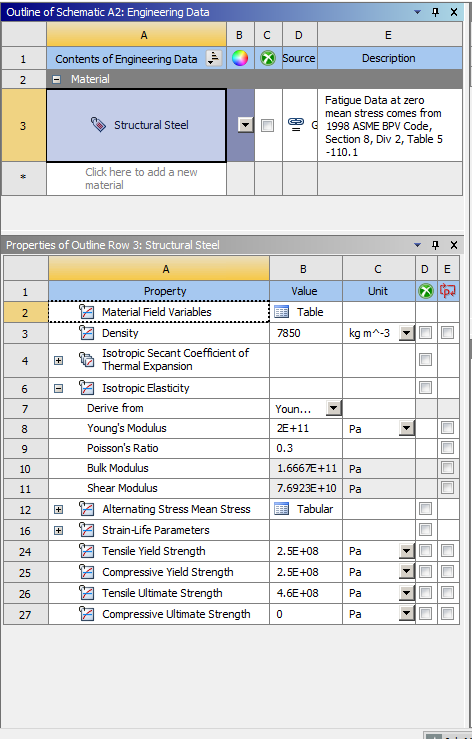
\includegraphics[height = 12cm]{./img/materials.png}
    \caption{Screenshot from ANSYS, showing the material selected for the spring and associated properties.}
    \label{fig:ansys1}
\end{figure}
\subsection{Load specifications used in FEA}
A vertical load was placed on the coil to simulate the compression forces that are imposed to it during its lifespan. This load was determined by considering the total static preload and cyclic superimposed loading that is applied onto the coil. The static preload is a proportion of the weight of the car, whereas the cyclic superimposed loading is the loads caused by driving maneuvers and surface roughness.   

The static preload is set at \SI{3720}{\newton} for this simulation, based on a quarter of the average weight of sedans (\SI{1519.53}{\kilo\gram} in the year 2020 \cite{b1}. The cyclic superimposed loading is set at 15\% of the static preload to imitate typical road conditions that the coil experiences most of its lifespan.
\subsection{Stress analysis results}
From the FEA conducted on ANSYS, the results seen in Figure \ref{fig:deformation1} and \ref{fig:stress1} were produced. We can observe that the stress experienced by the entire coil is rather even, with the inner sections of the coil experiencing marginally higher stress compared the outer sections. The maximum stress recorded was \SI{2.1e8}{\pascal}, lower than the compressive yield strength of structural steel.  
\begin{figure}[H]
    \centering
    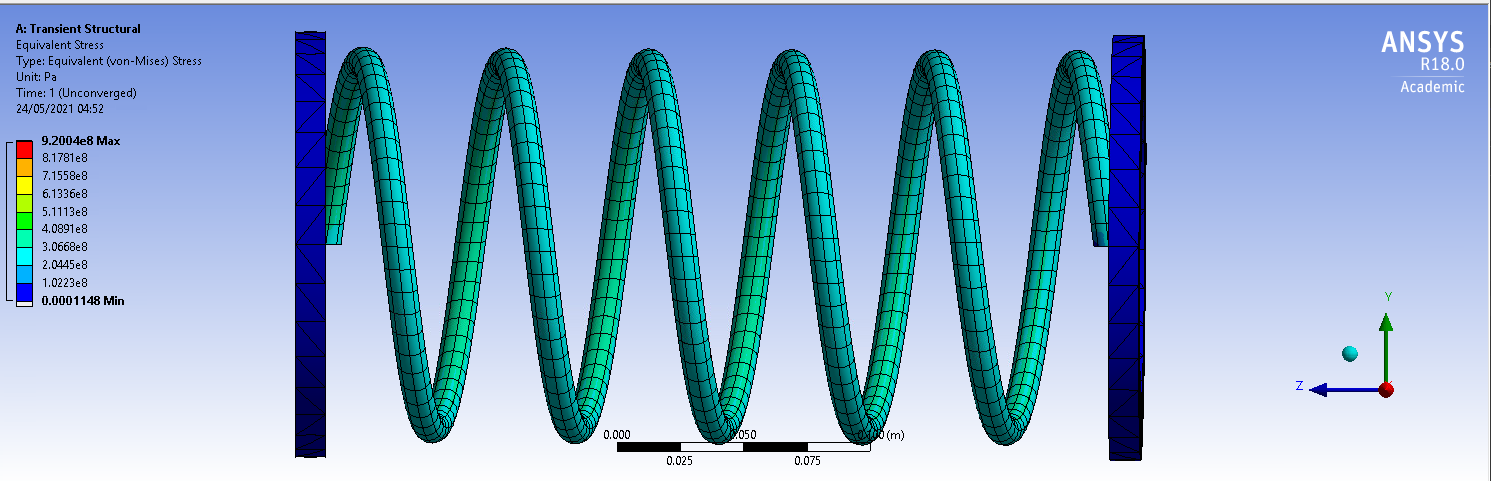
\includegraphics[height = 4cm]{./img/springanalysisvonmises.png}
    \caption{Screenshot from ANSYS, showing the stress in the spring when under load.}
    \label{fig:deformation1}
\end{figure}
\begin{figure}[H]
    \centering
    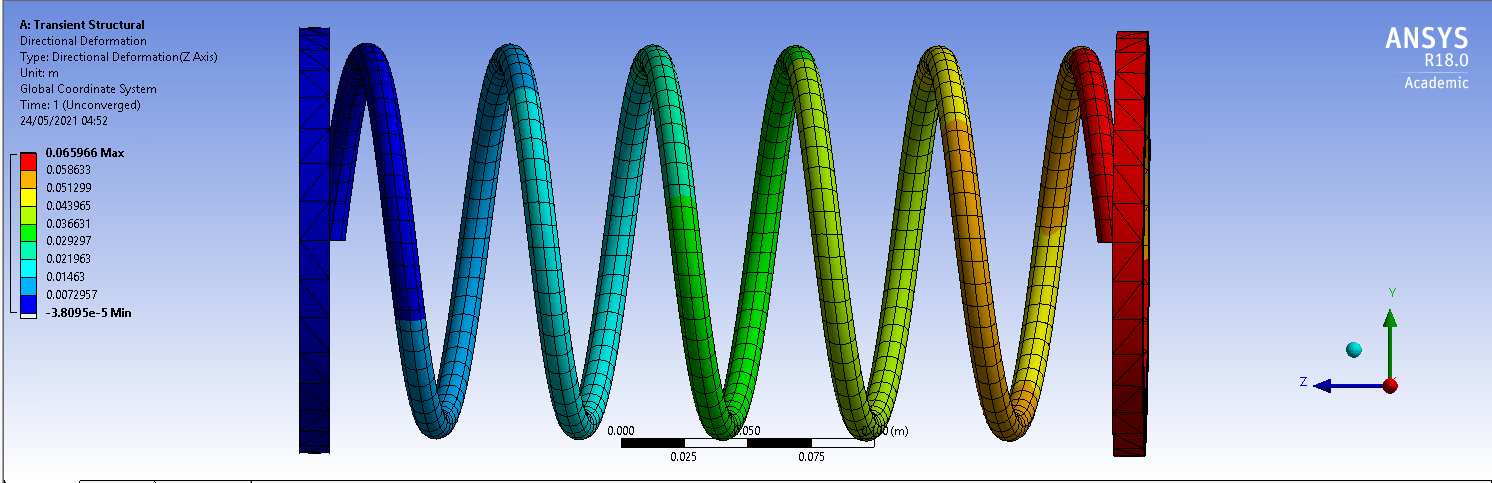
\includegraphics[height = 4cm]{./img/springanalysisdisplacement.png}
    \caption{Screenshot from ANSYS, showing the deformation in the spring when under load.}
    \label{fig:stress1}
\end{figure}
This indicates that under normal circumstances, the stresses experienced by the coil are not sufficient to cause failure. Therefore, it can be deduced that the cause of failure – fatigue crack arose due external factors that may have produced a stress concentrator on the coil. Due to the nature of the surroundings of the coil, the layer of paint protecting the steel may have been damaged from an oncoming object while the vehicle was moving or due to poor maintenance conducted, allowing corrosion to occur within the layer of paint that was meant to protect the coil.  

A fatigue crack would as a stress riser while attached to a vehicle, which amplifies the stress around the crack region significantly which leads to large stresses beyond the material ultimate tensile strength and eventually failure \cite{b2}.
\newpage
\section{Manufacturing analysis}
From research and of this type of coiled compression springs used in vehicle suspensions systems and overall inspection of our spring, there is a standardized method of manufacturing which includes, cold forming, heat treating and finally surface finishing \cite{b3}.

It is evident from the microstructure of the spring that it has been quenched and tempered as the microstructure shows fine martensite laths. From the material analysis, we have discovered that the carbon content is about 0.8\% which means it has a composition of 50:50 ferrite and pearlite. Therefore, this is consistent with the notion that the spring is manufactured from a steel that is quenched and tempered to obtain a desirable high strength that it needs to maximise elastic deflection to support the shock loading of the vehicle’s suspension.
\begin{figure}[H]
    \centering
    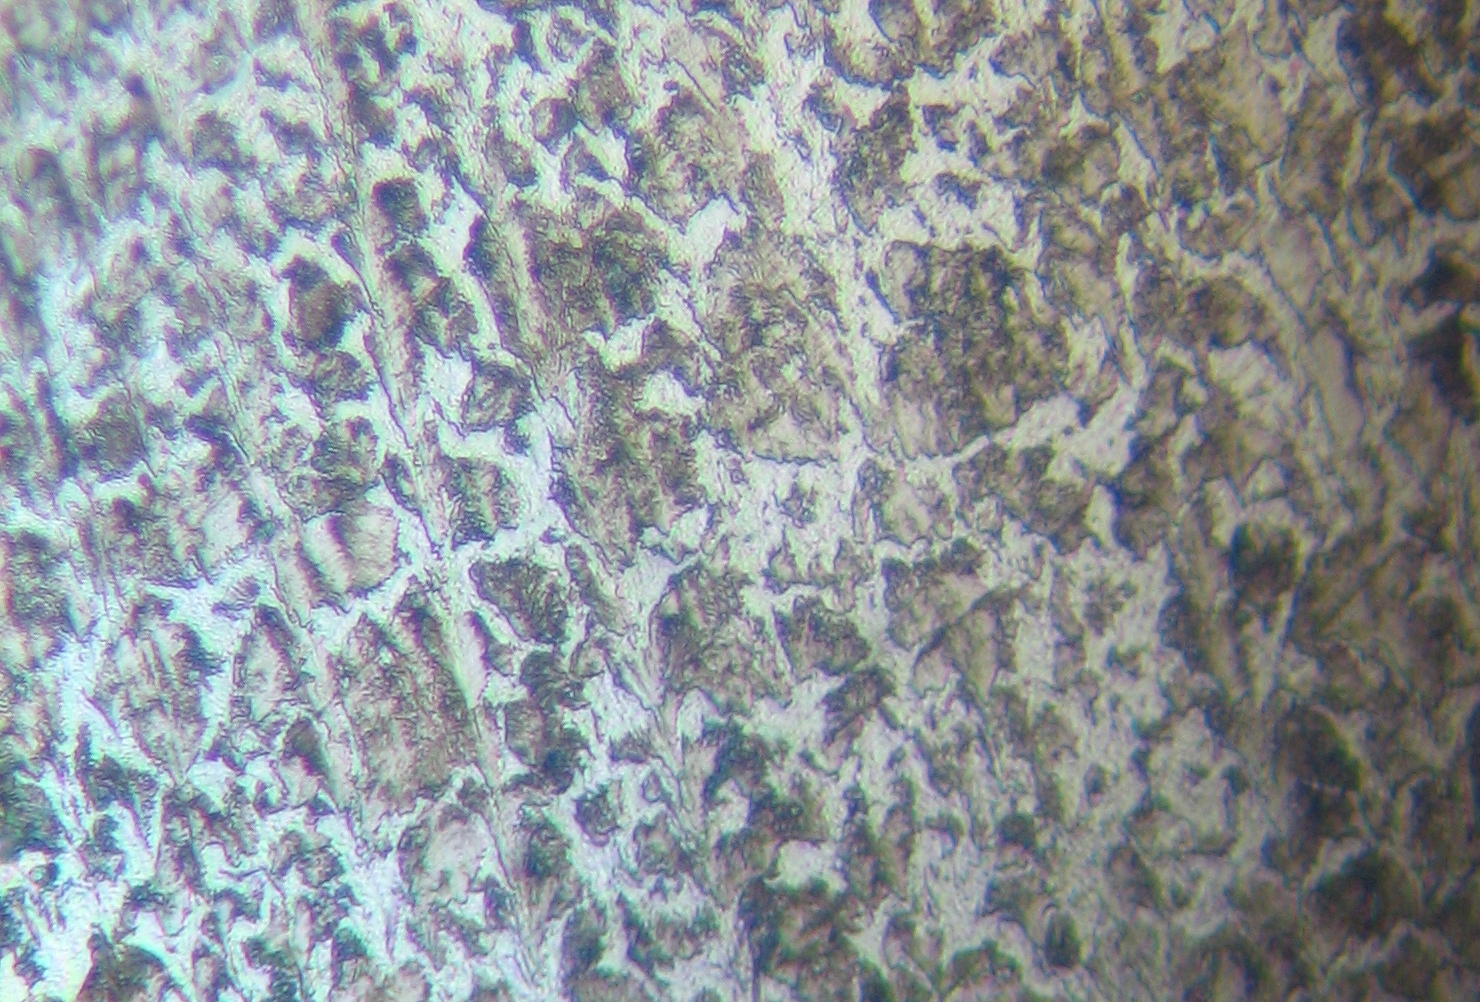
\includegraphics[height = 5cm]{./img/microstructure1.jpeg}
    \caption{Microstructure of spring steel that has 0.8\% carbon content and has a 50:50 ferrite to pearlite ratio.}
    \label{fig:microstructure1}
\end{figure}
\subsection{Raw material}
The raw material comes in large spools of high-quality spring steel. Based on our analysis of the spring, an annealed steel (that is unquenched) is used as there is evidence of subsequent heat treatment. The steel is then hot worked in order to draw them out into long wires. This is evident from the crystalline structure of the steel which shows that they are aligned along the axis of the spring. These spools are then unwound and fed into a cold forming spring coiler.
\begin{figure}[H]
    \centering
    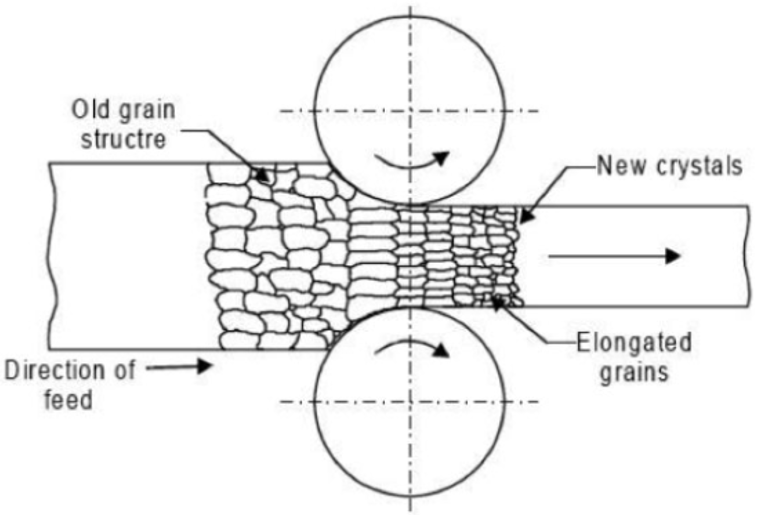
\includegraphics[height = 6cm]{./img/drawing1.png}
    \caption{Drawn out wire schematic showing that crystals align along the axis \cite{b4}.}
    \label{fig:drawing1}
\end{figure}
\begin{figure}[H]
    \centering
    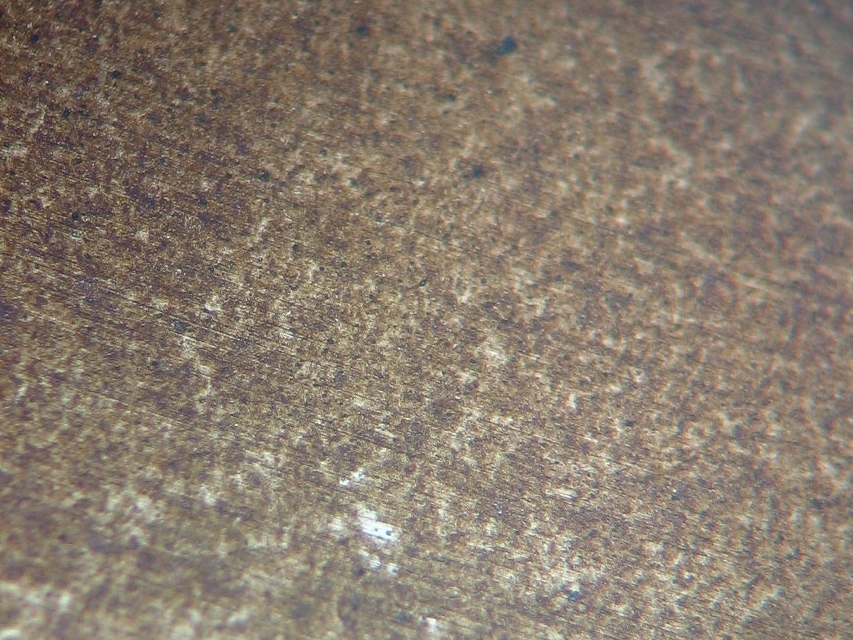
\includegraphics[height = 7cm]{./img/microstructure2.jpeg}
    \caption{Crystal structure of the spring showing that it is also aligned along the axis confirming that the wires were first drawn out.}
    \label{fig:microstructure2}
\end{figure}
\begin{figure}[H]
    \centering
    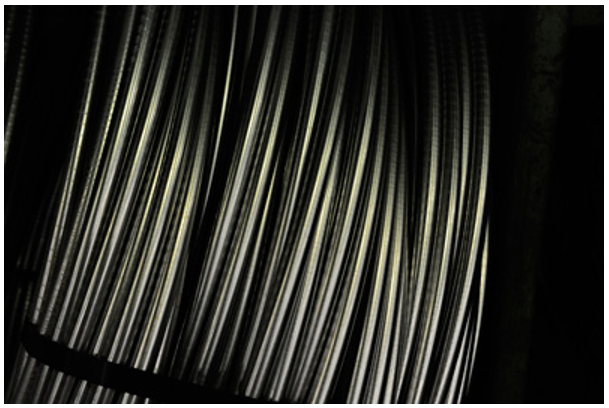
\includegraphics[height = 7cm]{./img/spools1.png}
    \caption{Large spools of drawn wire arrive at the factory for subsequent manufacturing.}
    \label{fig:spools1}
\end{figure}
\subsection{Cold forming}
Automatic machines firstly unwind the large spool of steel wires and straighten them out. The steel wire is then cold formed into a spring shape using an automatic coiling machine. Different from hot coiling where the wire has to be coiled around a shaft and requires a specific mandrel tool for each design, this method of cold forming the springs allow easy variation of the coil diameter, pitch and number of coils. Cold forming forces the steel beyond its yield (elastic) limit and the spring will retain its shape after removed from the coiling machine \cite{b5}. However, careful calibration is done to ensure that the steel is not forced beyond its tensile strength to prevent any fractures. This method of forming is also almost 100\% efficient as there is no scrap metal and all the material is converted into the end product.
\begin{figure}[H]
    \centering
    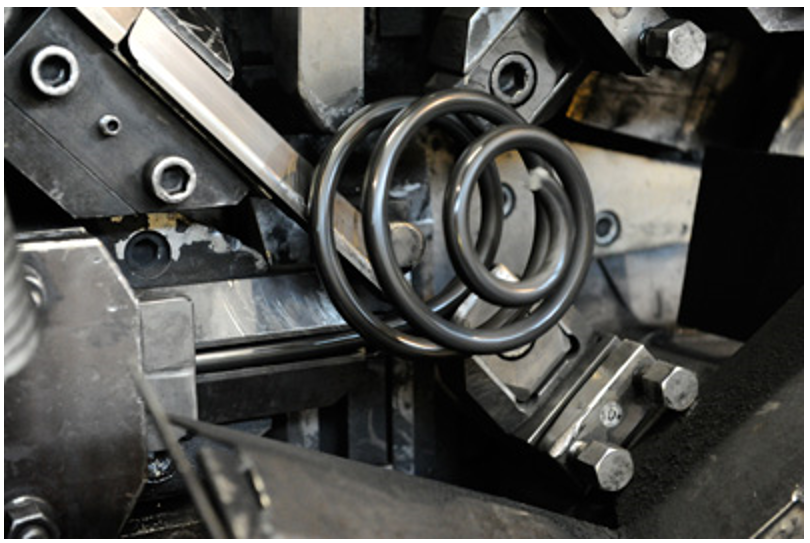
\includegraphics[height = 6cm]{./img/forming1.png}
    \caption{Cold forming spring coiling machine.}
    \label{fig:forming1}
\end{figure}
\subsection{Heat treatment}
As a result of the cold forming process, negative internal stresses are introduced into the steel. These can be removed using a stress relieving heat treatment followed by a hardening and tempering process to achieve the exact properties intended for the use of this suspension spring.
\begin{figure}[H]
    \centering
    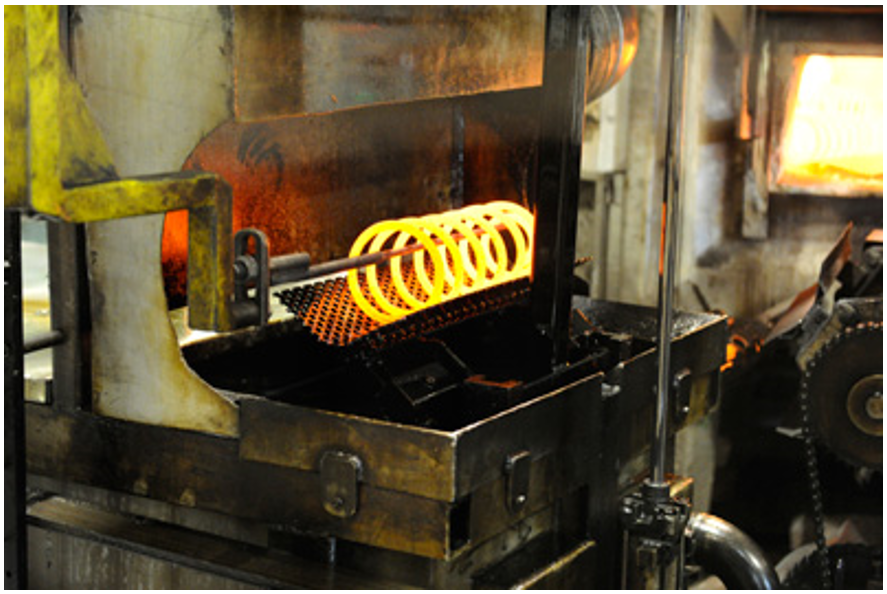
\includegraphics[height = 6cm]{./img/hotspring1.png}
    \caption{Spring being heated up for heat treatment process.}
    \label{fig:hotspring1}
\end{figure}
\begin{figure}[H]
    \centering
    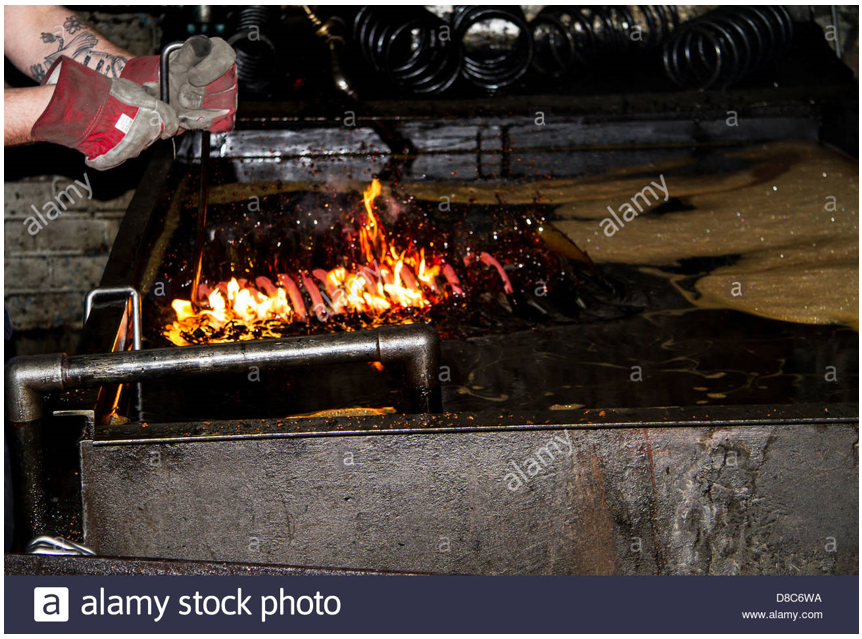
\includegraphics[height = 6cm]{./img/hotspring2.png}
    \caption{Spring being quenched for the tempering and hardening process \cite{b6}.}
    \label{fig:hotspring2}
\end{figure}
\subsection{Shot peening and presetting}
The shot peening and presetting process is then done in order to introduce and control the amount of required positive residual stress in the material. This positive residual stress reduces the sheer stress in the spring during compression and thus improving the spring performance as per requirement. This presetting operation is also known as the scragging operation which involves compressing the spring to introduce a positive residual stress.
\begin{figure}[H]
    \centering
    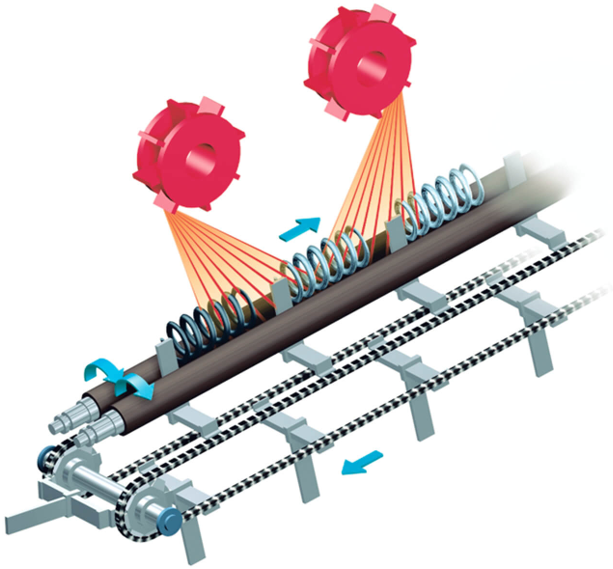
\includegraphics[height = 7cm]{./img/shotpeening1.png}
    \caption{Shot peening process where spring is bombarded by high velocity rounded particles \cite{b7}.}
    \label{fig:shotpeening1}
\end{figure}
\begin{figure}[H]
    \centering
    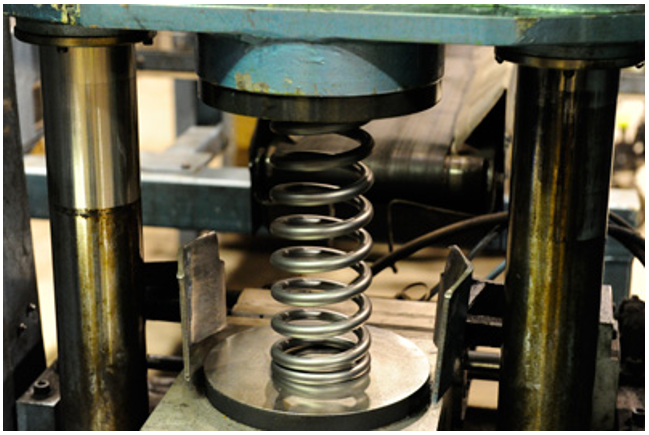
\includegraphics[height = 7cm]{./img/preset1.png}
    \caption{Presetting the spring to introduce positive residual stress.}
    \label{fig:preset1}
\end{figure}
\subsection{Surface finish}
For increased corrosion resistance, the springs are subjected to galvanizing using zinc phosphate before painting. The surface of the spring is then protected from the elements with an epoxy powder coating that is sprayed onto the surface using a spray paint gun. It gives a more consistent finish and is more resistant to chipping, scratching and other forms of wear due to the thermal bonding it undergoes during the curing process \cite{b8}.
\begin{figure}[H]
    \centering
    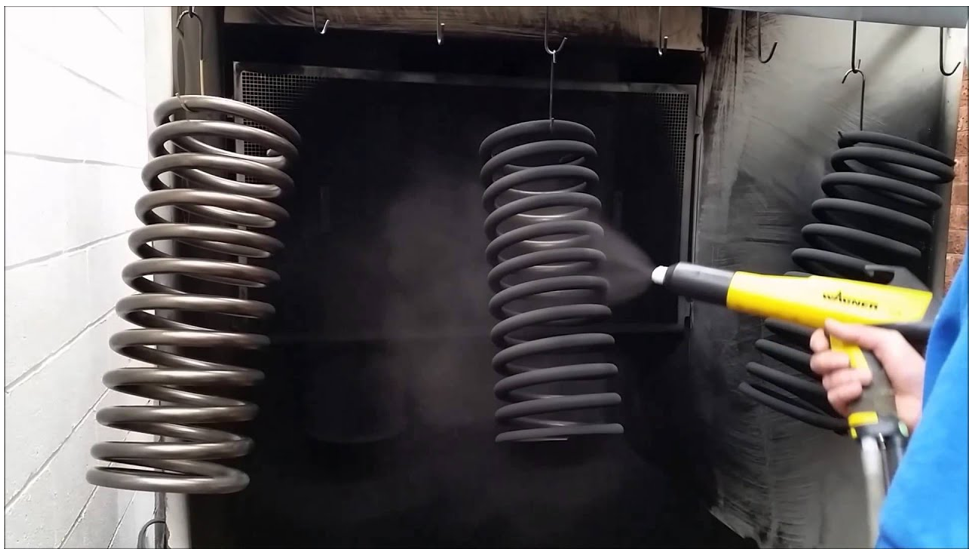
\includegraphics[height = 8cm]{./img/spray1.png}
    \caption{Powder coating being applied onto a suspension spring \cite{b9}.}
    \label{fig:spray1}
\end{figure}
\subsection{Defects that arise from the manufacturing process}
Cold forming can come with a host of defects that may change the global properties of the steel used to make these suspension springs. Some of these defects include:
\begin{itemize}
	\item Fractures: Cracks can form both on the surface and internally usually caused by more stress or friction than the material can handle.
	\item Surface imperfections: Roughness, scratches and scoring are examples of surface imperfections that can be introduced by cold forming. These will act as stress concentrators and ultimately cause the material to fail before the estimated lifespan as crack propagation occurs leading to fracture.
	\item Flow imperfection: These include problems such as folding, under filling, flashes and buckling.
	\item Changes in properties: Although rare some examples of this includes decarburization and formation of martensite. 
\end{itemize}
Other defects that may arise from the heat treatment process include oxidation, decarburization, fracture and warping \cite{b10}.
Although there was potential for defects to be formed during the manufacturing process, the spring examined had no signs of major flaw that was due to the forming and subsequent heat-treating processes. The one weakness was probably the durability of the epoxy powder coating that failed to shield the inside of the spring from moisture and allowed corrosion to take hold onto the part. (This will further be explained in the following section)
\newpage
\section{Material analysis}
The material analysis would suggest the composition, hence the properties of the material making up the spring in order to help with further analysis.
\subsection{From the designer's point of view}
This is one of the 4 springs from a car suspension system, which therefore supported at least ¼ of the weight of the car, plus the absorption of the varying vertical acceleration while the car is driven. Figure 1 shows the analysis of the resultant shear stresses that the compressive spring experienced while it is loaded. It is the combination of the direct and the torsion shear stress. So, this material selected by the designer should be high in toughness in order to withstand the many cycles of large loads. The desirable high strength is to maximise its elastic deflection which absorbs these impacts. Meanwhile, as a component of a mass-produced type of vehicle, it suggests that this should be a material that is low in both the cost of the material itself and the cost of manufacture, as well as its ease of manufacture.
\begin{figure}[H]
    \centering
    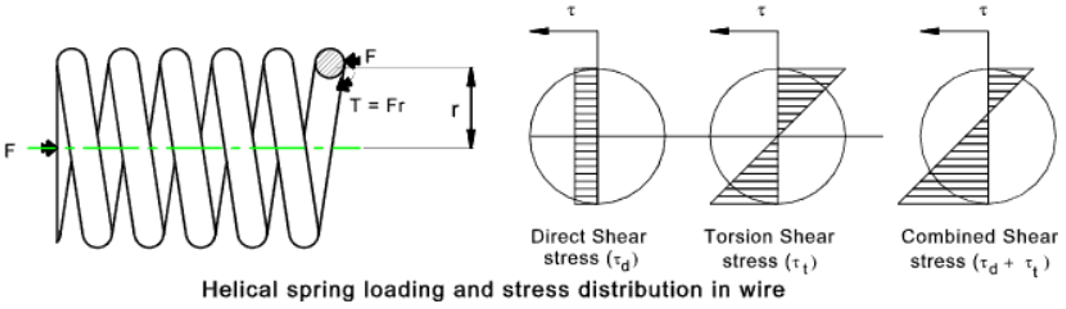
\includegraphics[width = \textwidth]{./img/helical1.png}
    \caption{The stress of the loaded spring \cite{b11}.}
    \label{fig:helical1}
\end{figure}
\subsection{The material and its heat treatment}
The corrosion patterns on the surface of the spring, the reddish-brown oxide is shown in Figure \ref{fig:rust1}, is rust. This is formed by the reaction of iron with oxygen, which is also called oxidisation, usually presences in water or moist air mixture. The chemical equation is The chemical equation of the formation of the rust is \ce{4Fe + 3O2 + 6H2O -> 4Fe(OH)_3}. This reaction consists of two steps. The first step is the dissolution of the solid iron in the water, \ce{Fe(s) -> Fe^{2+}(aq) + 2e^-}. For the second step, the reaction of \ce{Fe^{II}} and hydroxide \ce{(OH^-)} ions in the water \ce{Fe^{2+}(aq) + 2OH^-(aq) -> Fe(OH)_2(s)}, produces the green rust. Also, this reaction produces the \ce{Fe^{III}} ions, as \ce{4Fe^{2+}(aq) + 4H^+(aq) + O2(aq) -> 4Fe^{3+}(aq) + 2H2O(l)}. The \ce{Fe^{III}} will then combine with extra hydroxide, \ce{Fe^{3+}(aq) + 3OH^-(aq) -> Fe(OH)_3}, which forms the \ce{Fe^{III}} hydroxide. This then dehydrates to become rust. 
 
Combining with the analysis from the first part, it suggests that the spring is made of steel instead of pure iron since the iron is too soft to match its design requirements.  
\begin{figure}[H]
    \centering
    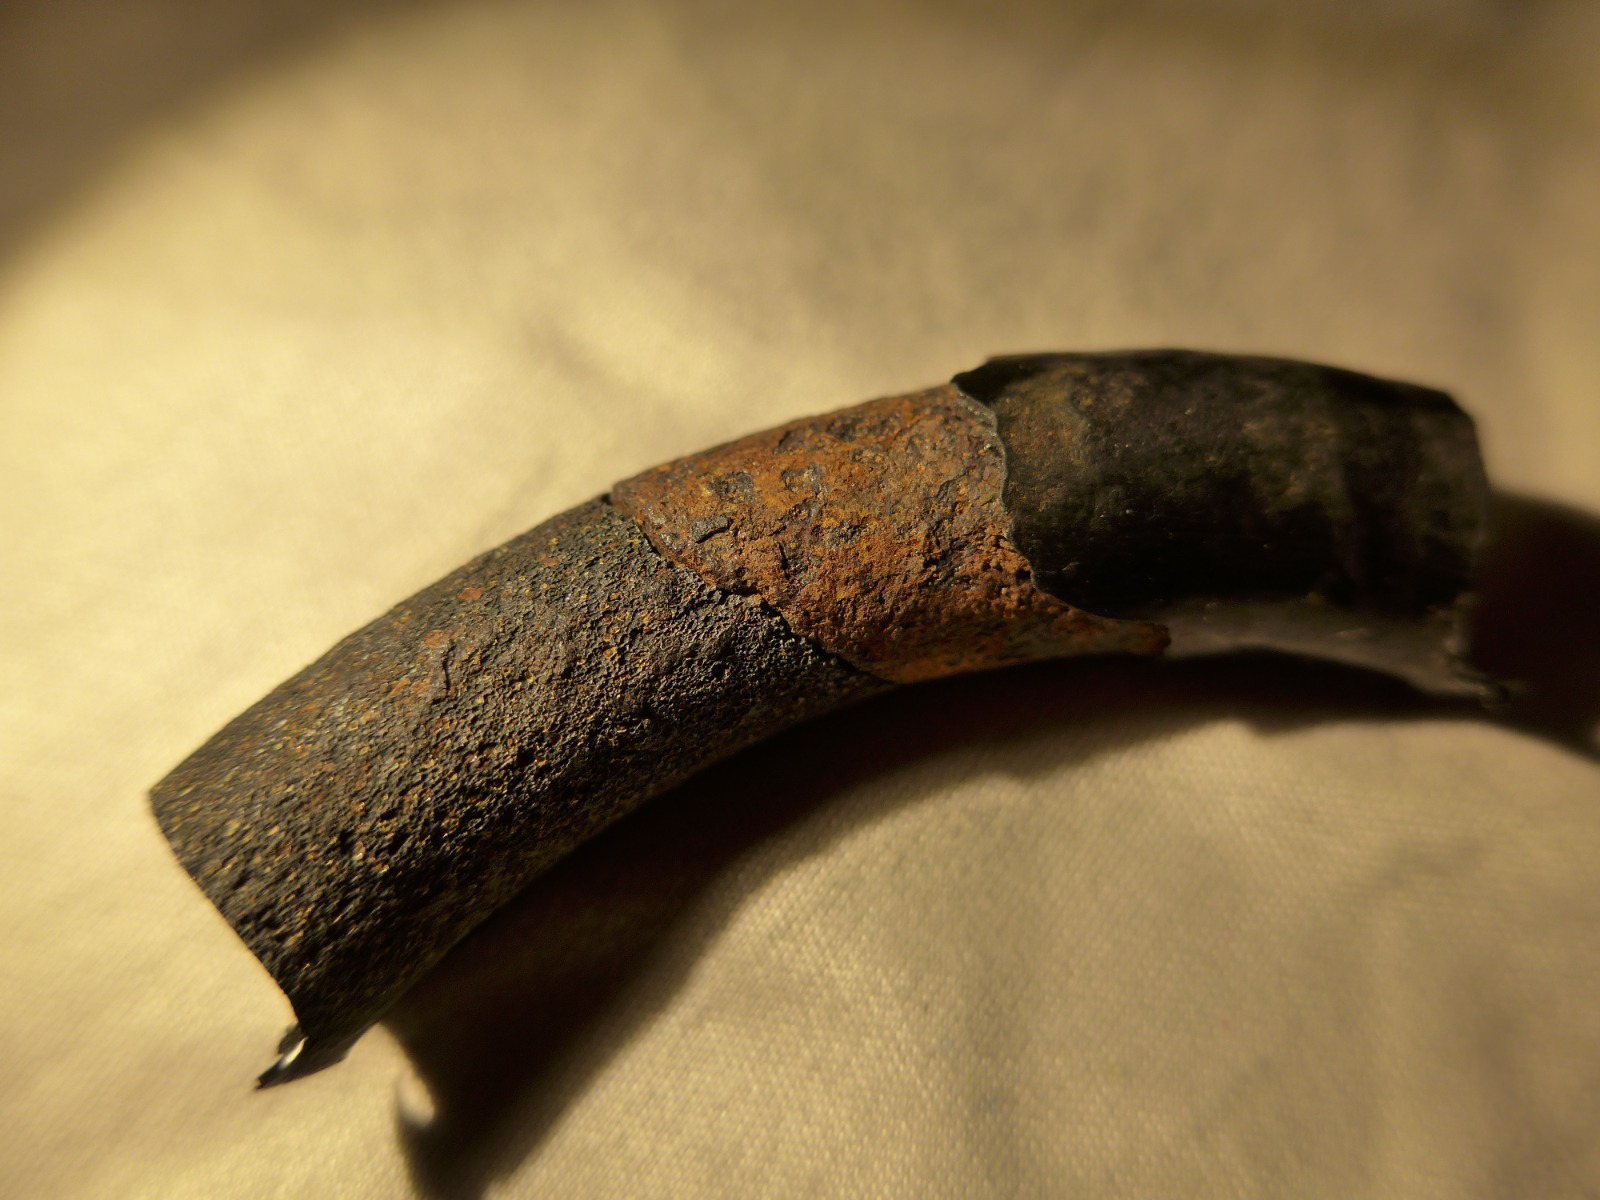
\includegraphics[height = 7cm]{./img/rust1.jpeg}
    \caption{The corrosion patterns on the surface of the spring.}
    \label{fig:rust1}
\end{figure}
Figure \ref{fig:microstructure3} is the microstructure of the cross-section at a magnification of 100, which was polished and etched conventionally in Nital, to find out what composition the steel was. This indicates that the steel is a quenched and tempered steel. The microstructure shows fine martensite laths, which tells that there has been a very rapid cooling process. And this means that the material was almost definitely quenched. At the same time, because the spring must be tough enough, as the discussion in part 1. Therefore, the spring was also tempered in order to retain the hardness given by the quenching process, meanwhile, increase its toughness and fracture toughness ($K_c$). The fracture has little plastic deformation, which suggests that the tempering may not be so strong, though it is hard to determine the exact level of the tempering. 
\begin{figure}[H]
    \centering
    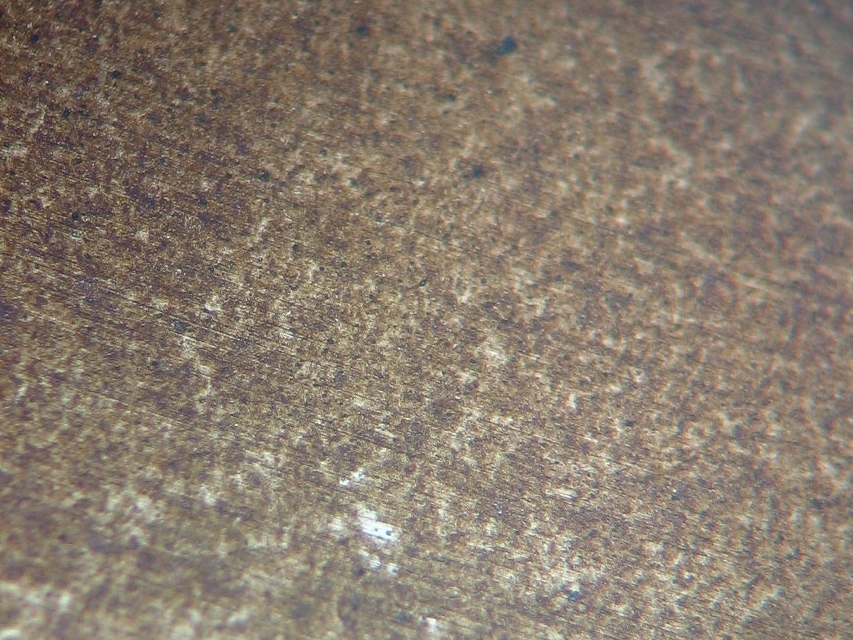
\includegraphics[height = 7cm]{./img/microstructure2.jpeg}
    \caption{Microstructure of the cross-section.}
    \label{fig:microstructure3}
\end{figure}
What is more, there is an apparent orientation on the structures that occurred, which direction is along the axis of the road. This may also suggest that the material has undergone other hot working before the heat treatments. 
\subsection{Composition analysis of the steel}
For the microstructure analysis, the heat treatment of the spring needs to be ‘removed’ to recover the original microstructure. This piece of material was heated up to about \SI{700}{\celsius} using a blow torch and allowed to cool slowly. The slow cooling should give the equilibrium microstructure. The x100 magnified cross-section is then shown in Figure \ref{fig:microstructure4}, which could help to get the carbon content of the steel. The specimen was etched in Nital. The pearlite has a lamellar structure with alternating layers of two phases, the ferrite and the cementite. Because the cementite looks darker after etching, the pearlite is then shown as the darker patches in Figure \ref{fig:microstructure4}. Hence the ferrite is shown as the lighter regions. So, from Figure \ref{fig:microstructure4}, it appears that the ratio of ferrite to pearlite is about 50:50.
\begin{figure}[H]
    \centering
    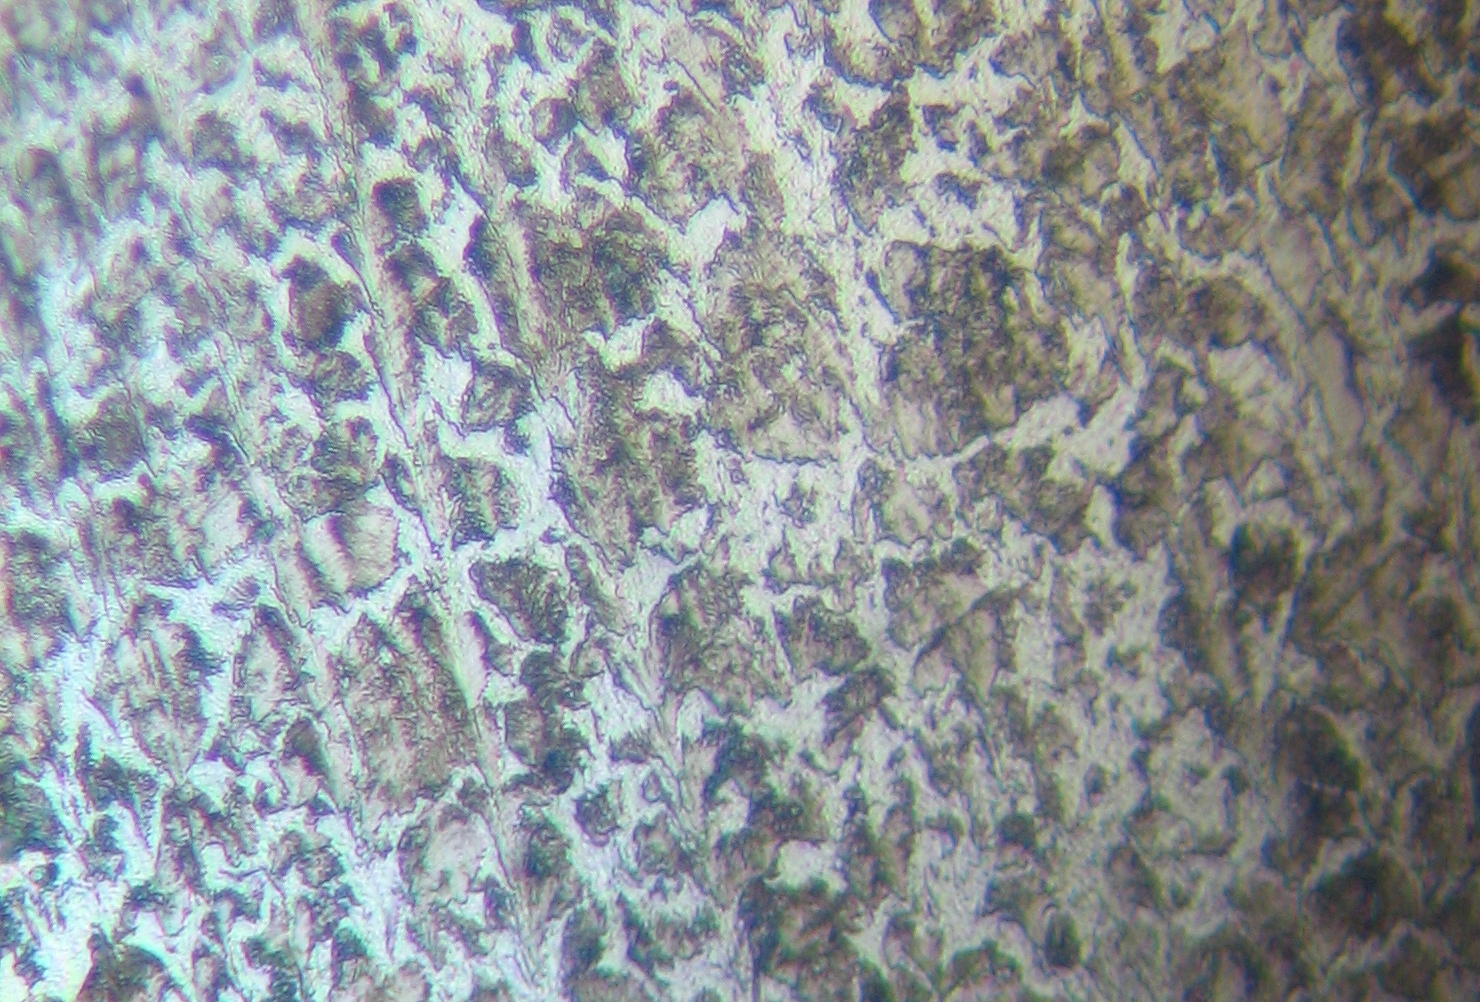
\includegraphics[height = 6cm]{./img/microstructure1.jpeg}
    \caption{The microstructure after etching in Nital and ‘removing’ of the heat treatment.}
    \label{fig:microstructure4}
\end{figure}
And therefore, checking the corresponding carbon content in the phase diagram of Figure \ref{fig:phasediagram}, it is about 0.8\% (0.83\%). At this eutectic point, the pearlitic microstructure has the most layers of ferrite and cementite, which helps to prevent the propagation of the dislocation. This material is strong and cheap steel, which allows the subsequent heat-treatment after drawing to the rod and then forming the coil. 
\begin{figure}[H]
    \centering
    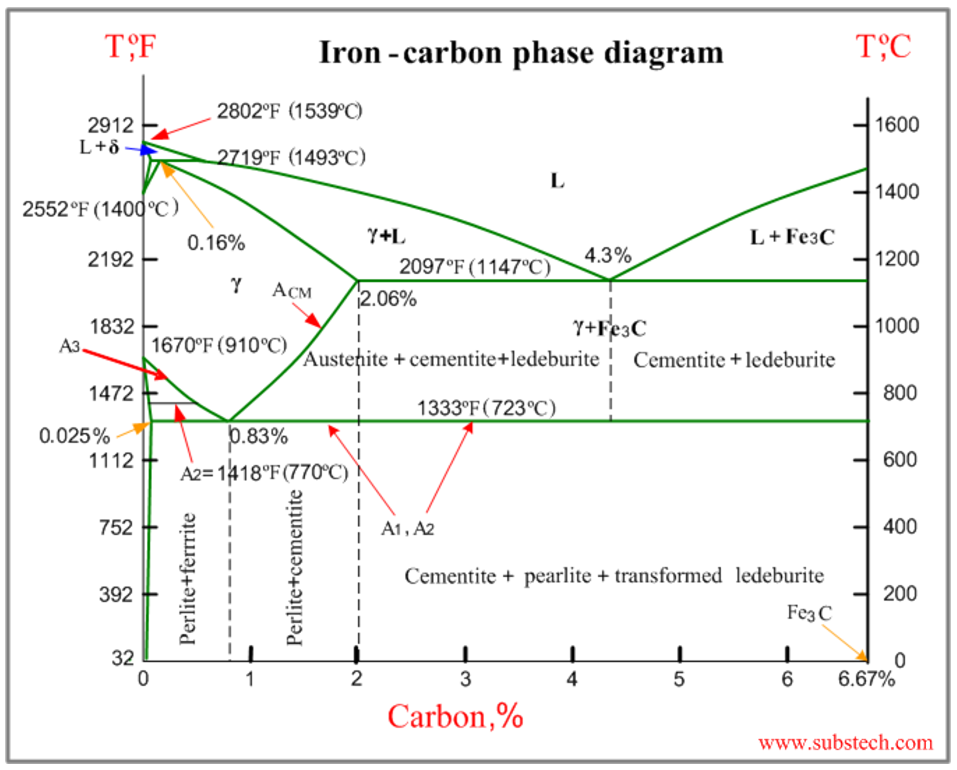
\includegraphics[width = 0.6\textwidth]{./img/phasediagram.png}
    \caption{The phase diagram of iron-carbon \cite{b12}.}
    \label{fig:phasediagram}
\end{figure}
A simple portable hardness tester is used to measure the Vickers hardness of the specimen. It was about 550 VPN, and the approximate tensile strength is $550\times 2.8 = \SI{1540}{\pascal}$. This value is very high, with the contribution of the quenching and tempering processes, and would satisfy its design requirements. In addition, this may also suggest that it might have undergone extra work-hardening processes.
\subsection{The surface protection}
The corrosion is severe, as shown in Figure \ref{fig:rust1}. The paint on the surface is heavily damaged. It is likely to be difficult for the suspension system to be dry since it is located under the car in a semi-closed environment. The moisture remains in the air, which raised the rate of corrosion.  
 
The coating of paint is the most widely used material to coat and protect steel. The cost of paint is low, which is suitable for this application. It works as a boundary, which separates the steel from the air, i.e. separating the reactants to prevent the chemical reactions. However, the paint can also be corroded, before the corrosion of the material inside. When a bit is removed, the blistering paint act as an incubator for more corrosion. 
\subsection{Summary}
The analysis of the material suggests that the spring is made of steel which contains about 0.83\% carbon and experienced the quenching and tempering process. It is suspected that it may have undergone other heat-working before the heat treatment and extra hardening process. Its ratio of ferrite to pearlite is about 1:1, and the tensile strength approximated is \SI{1540}{\pascal}. These made the spring high in strength, hardness, and toughness. The coating is severely damaged, but it was determined to be the paint, due to the left-out paint pattern shown in Figure \ref{fig:microstructure3}. This material analysis provides more information on the physical properties of the material, the manufacturing processes it undergoes, and implies some clues of the failure.
\newpage
\section{Failure mechanisms}
The reason of failure of the steel suspension spring from a car is due to fracture. Defects come from fatigue processes, existing manufacturing faults, corrosion along grain boundaries and cavities from internally that join to form cracks called creep. 
\subsection{Corrosion}
One possible cause of failure is corrosion on the surface of the spring, as the material (steel) tends to rust easily. Corrosion occurs due to the interaction of the material with its environment, leading to a loss of the material. Corrosion on the surface combines with other types of failure, such as fracture and fatigue, and can worsen them. A coating such as paint is used to protect the surface and prevent corrosion. The flexibility of the paint allows it to withstand and adhere to the surface even under the compressive movement of the component. However, this property is limited to the expected range of loading on the part, impurities, acidity and temperature. Use of the paint longer than the expected lifespan can be the cause in the long term. Moreover, any careless handling of the component by a technician or user can be the reason for coating failure in a shorter time.  
  \begin{figure}[H]
    \centering
    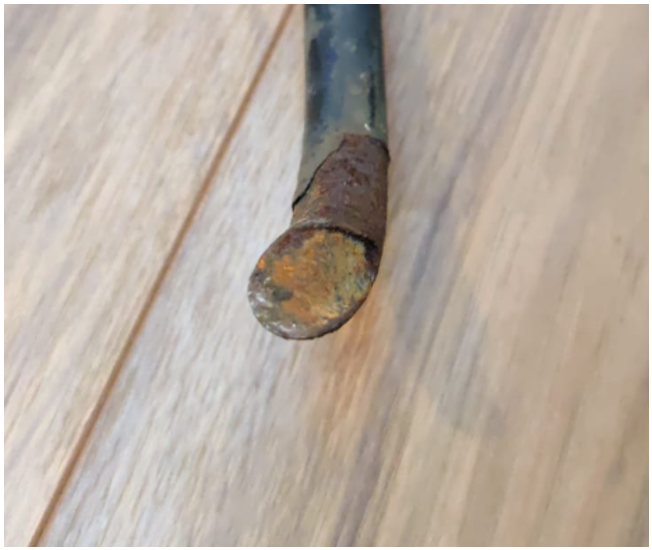
\includegraphics[height = 8cm]{./img/fracture1.png}
    \caption{Fracture surface.}
    \label{fig:fracture1}
\end{figure}
One of the mishandling would be the overloading on the component, such as compression for suspension spring. Over-compression due to a large number of road bumps or going over the bump with non-ideal speed could lead to a collision and abrasion between coils. Collision over time may have caused thinning of the paint and eventually exposed the component’s surface. A single deep scratch due to the collision could have also caused surface exposure. The exposure of the surface to both water and oxygen in the atmosphere and direct contact could have led to corrosion—initiation of the corrosion results in the propagation on the whole surface of the spring. In Figure \ref{fig:fracture1}, the corrosion on the fracture surface can be shown. The corrosion on the existing hole or crack surface could have accelerated the weakening of the steel structure and cause a further crack and corrosions. Another possibility is the presence of corrosion pits, an area with greater rate of corrosion. From these pits, corrosion at grain boundaries could have initiated the cracks and further corrosions on the surface. The crack gives the site of stress concentration resulting fracture of the component. 

Direct contact with water could have occurred if we consider the position of the suspension spring and the presence of a drainage tray. The component is placed at the bottom part of the car where the coil is exposed to rain and water splash. The tray is used to protect the suspension spring from impurities such as dirt and placed next to the component. It has small holes to drain the water or tiny contaminants. However, because of the size of the hole, it may clog with impurities collecting water and other impurities in the tray. The salt from the road could have accumulated in the tray with water and act as an electrolyte allowing easy flow of the electrons.  
 
Corrosion cannot be the only reason and factor that contributed to the failure but one of initiative or accelerator of the fracture. Environmental factors such as direct contact with water or temperature could have also been the initiative to the failure as these could initiate corrosion. These factors are synergistic, and each mechanism enhances each other beyond what damage would normally be expected to occur. 
 
To prevent corrosion from occurring, the only way is to coat the surface. The use of polymer paint that has the flexibility to move along with the motion of the spring may decelerate the initiation of the corrosion. Another factor that can be considered for the prevention is driving in an ideal condition: preventing any sudden shock to the car. A lot of sudden motion change and collision of the car is caused by the user driving fast over the road bump causing a sudden large shock to the coil. Careful and standard driving could prevent the thinning of the paint and corrosion on the surface. Furthermore, constant clean-up of the drainage tray can prevent the accumulation of salt and water near the suspension coil. 
\subsection{Fatigue fracture}
The failure of the suspension spring from the car could be due to various factors. The failure could be due to fatigue fracture, as the spring experiences a cyclical load - that is a load that varies in time. Fatigue is a phenomenon that is associated with variable loading or cyclic stressing or straining of a material. It is like us humans getting fatigue when a particular task is repeatedly performed. Similarly, metallic components such as the steel suspension spring that are subjected to variable loading get fatigue, leading to premature failure under certain conditions. The cyclic load on the suspension system of the vehicle can cause failure as it initiates the formation and growth of a new crack, or it causes crack growth of an already existing crack with repeated loading. Fatigue involves the initiation of defects (cracks)- if one occurs naturally, followed by the propagation of these, until the critical crack size $a_c$ is reached at which point failure then occurs by fracture. Impurities and discontinuities in the microstructure do seem to assist fatigue as they act as stress concentrators. 
 \begin{figure}[H]
    \centering
    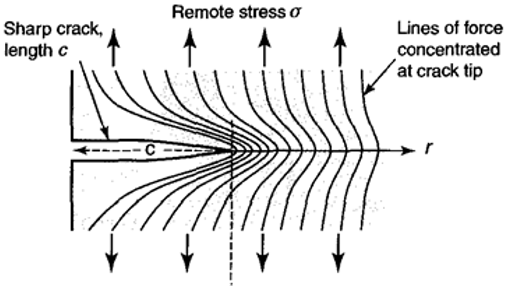
\includegraphics[height = 5.5cm]{./img/stress1.png}
    \caption{Stress concentration around the crack tip \cite{b13}.}
    \label{fig:stress2}
\end{figure}
The fracture of the spring developed due to localized stress which introduces stress concentrators at a particular point on the coil of the suspension spring. The stress concentrators that lead to the crack could be in the form of sharp edges, machined holes, scratches, dents, machining marks, material defects, grain boundaries or in our particular case corrosion pits. The fatigue crack growth mechanism, for an existing defect in the spring material, is when the stress concentration increases, $\sigma$, the crack opens and the localised stress ($\sigma_{local}$) increases to be greater than the global stress ($\sigma_{global}$) induced by the load supported, but limits at $\sigma_Y$, because any higher is not possible as yielding occurs first. The area of high concentration around the crack tip reaches $\sigma_Y$ generating plastic deformation locally which creates extra surface internally. When the cycle moves into compression, the extra surface will have to be folded inwards and extends the crack in the process. This process repeats for each cycle and the crack propagates giving striations that is visible under very high magnitude on an electron microscope. Therefore, the mating surfaces are very flat, and this generate hair-line cracks which are difficult to spot. The cracks will grow until fast fracture occurs as the crack gets to critical crack size $a_c$ which causes the coil to fracture. As this happens in the coil of the spring the fractured surface is indicative of fatigue. Beach marks are created because of minor variations in the loading cycle, for example changes in stress amplitude ($\sigma_a$), mean stress ($\sigma_{mean}$), maximum stress ($\sigma_{max}$) and minimum stress ($\sigma_{min}$). The beach marks are also a positive indication of fatigue. 

Fatigue cracking has three phases. In the first phase of the fatigue cracking is called stage I, include crystal chips which extend through contiguous grains and surface imperfection, playing a role in crack formation. The cracks can also be initiated by nucleating slip planes, notches and internal flaws in the spring material. During the dynamic loading, work hardening on one of the planes due to the motion of dislocations could occur hence increasing local stress and on return cycle, slip is unlikely to occur on the same plane so slip occurs on another plane. The slip steps increase the surface roughness and the formation of embryonic cracks that act as stress concentrators which will initiate fatigue crack growth in the second phase. The cracks initially appear at \SI{45}{\degree}, which is where there is maximum shear stress for slip, and then turn to become \SI{90}{\celsius} to the applied maximum tensile load at the second stage. The second phase is called stage II fatigue which involves crack extension causing the atoms to become disconnected. The stress concentration becomes maximum at the crack tip. The advance of the crack is orderly and can be viewed on an electron microscope. The final fracture takes place during stage III fatigue. 
\begin{figure}[H]
    \centering
    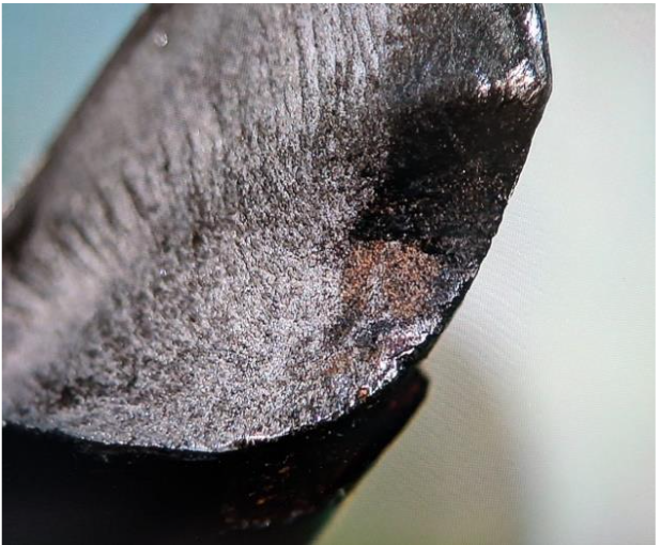
\includegraphics[height = 8cm]{./img/fatigue1.png}
    \caption{Fatigue failure of the coil with corrosion - bright, smooth regions show fatigue; darker and rough regions show fracture.}
    \label{fig:fatigue1}
\end{figure}
In the case of this car suspension spring, it always experiences a compressive load due to the weight of the car. There are dampers present to ensure that the motion of the spring is smoothened and to ensure that it does not move vigorously up and down which could cause damage from fatigue crack growth. However, the fatigue crack can grow due to the presence of residual stress. As the compressive load can generate a residual tensile stress at the crack tip, which helps the external stress to propagate the defect. In this case, a single underload can reduce lifetime of the spring so fewer cycles are required to failure. Most engineering fatigue scenarios contain existing defects, so we assume that the spring has an existing defect and the fatigue over time causes propagation.
\subsection{Manufacturing}
The faults during manufacturing processes causing crack-like defects which act as stress concentrators. This means the lifetime decreases as the imperfections in the manufacturing process causes cracks to initiate. 
\begin{figure}[H]
    \centering
    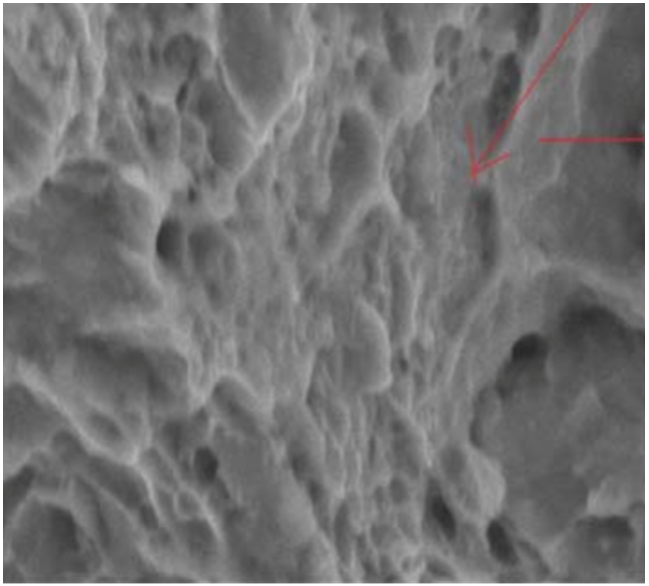
\includegraphics[height = 8cm]{./img/cracks1.png}
    \caption{Holes in the coil spring \cite{b14}.}
    \label{fig:cracks1}
\end{figure}
The small hole and crack on the surface causes imperfection which could be due to manufacturing or tempering process. Any hole or change in shape of the material can act to magnify global stress therefore help to initiate cracks. There could also be inter granular surface covered by an oxide due to trapped quench oil being heated in tempering furnace. The oxides trapped in the microstructure, can be angular and sharp in shape hence very effective stress concentrators. The defects cause the local yield stress to increase to become greater than the yield stress, causing failure to occur after a while. This type of defect takes place when the heating system was not properly done, the quenching crack and holes reduce the life of the suspension coil spring, hence causing premature failure.  
 

To design against fracture, the material of the coil has to be carefully selected as the engineers need to be aware of how these can either help or hinder fatigue crack initiation and propagation by paying careful attention to the quality of the supplied materials. They need to ensure that they consider the existing fatigue data and research on the material, as often small changes in alloy composition or specification can have commensurate change in fatigue properties.  
\subsection{Creep}
\begin{figure}[H]
    \centering
    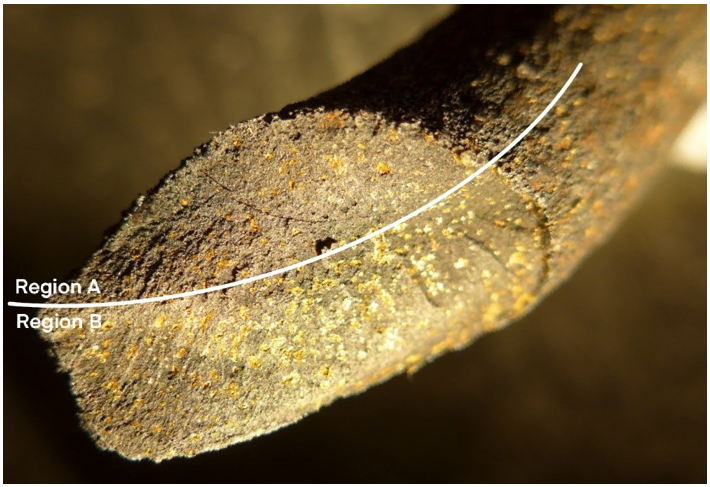
\includegraphics[height = 7cm]{./img/creep1.png}
    \caption{Surface of the fracture.}
    \label{fig:creep1}
\end{figure}
We can identify two regions with different surface patterns from the observations: region A with a smooth and flat surface and region B with a rough and ridged texture. Region A is smoother than region B suggesting brittle fracture in this region. This fracture occurs instantaneously below the maximum yield strength. Unlike region A, region B is not smooth, suggesting the possibility of ductile fracture and the cause of the crack. The chevron crack pattern of the surface indicates the direction of crack propagation. Combining these two regions, we cannot say it is a definite brittle fracture but more of a moderately ductile fracture. 

Creep is when the internally formed cavities join to form cracks. Creep occurs when the part plastically deforms below the yield strength over a long period. Several factors cause it, and one of the most influential factors is temperature. The temperature from the road and the car may have encouraged oxides to form and eventually initiate creep. The ridged surface and cracks until the critical length suggest the loading applied over a span of time. The compression and expansion of the spring when the car goes over the bump and a constant vibration from the car could have provided the long-term stress on the spring. This loading could have accelerated the crack and deformation on the spring and eventually resulted in a fracture. This factor, again, could have been influenced by the other factor such as manufacturing process and corrosion and affect other factors such as fatigue. 
 
To prevent creep, the driver can avoid driving over a road that may cause long term stress that is below yield strength. Other methods are used higher melting point metals as the temperature affects the creeping phenomenon. The material used can be changed with one with greater grain size because the thermomechanical process increases the grain size but decreases the creep rate.  
\subsection{Conclusion of failure}
There is no sign of the manufacturers not performing the manufacturing process of the suspension spring improperly and there is no sign that the material used for the spring is in anyway not the right choice, so we can only assume that the reason of the fracture was due to environmental factors like corrosion. Corrosion and corrosion pits on the surface of the spring could have initiated the crack providing a site of stress concentration accelerating other factors such as fatigue. In addition, the fatigue as the spring experiences a cyclical load could have initiated the crack and corrosion can influence fatigue crack. There could have been inconsistencies in the checking of the suspension springs where they could have detected the defect in the spring, as they check for corrosion so that the spring can be replaced before the crack propagates further. There are also non-destructive evaluation tests that are done to both detect defects and size defects which help to determine the remaining lifetime via a mathematical framework. Methods like X-ray inspection, ultrasound inspection, eddy-current methods, magnetic particle inspection and dye penetrant methods could be used to size the defects. This would allow for replacement of the spring, repair by welding or remove cracks by polishing.
\begin{thebibliography}{00}
    \bibitem{b1} "Highlights of the Automotive Trends Report | US EPA", US EPA, 2020. [Online]. Available: \url{https://www.epa.gov/automotive-trends/highlights-automotive-trends-report}. [Accessed: 24- May- 2021].
	\bibitem{b2} M. Decker, S. Rödling and M. Hück, "Suspension Springs – Experimental Proof of Reliability under Complex Loading", in 13th International Conference on Fracture, Beijing, China, 2013.
	\bibitem{b3} "Kilen Springs - Technical - Manufacturing", Kilensprings.com, 2021. [Online]. Available: \url{https://www.kilensprings.com/springs-production/coil-spring-manufacturing.asp}. [Accessed: 24- May- 2021].
	\bibitem{b4} Origin Media, "Understanding Grain Structure and Direction when Plate Bending", Barnshaws.com, 2021. [Online]. Available: \url{https://www.barnshaws.com/information/articles/understanding-grain-structure-and-direction-when-plate-bending}. [Accessed: 24- May- 2021].
	\bibitem{b5} "Cold Forming Principles", Nationalmachinery.com, 2021. [Online]. Available: \url{http://www.nationalmachinery.com/cold-forming-principals#:~:text=Cold\%20forming\%20is\%20a\%20high,amounts\%20of\%20material\%20by\%20trimming}. [Accessed: 24- May- 2021].
	\bibitem{b6} Alamy Limited, "Stock Photo - Coils suspension spring being lowered into oil quenching bath in a UK manufacturing company", Alamy, 2021. [Online]. Available: \url{https://www.alamy.com/stock-photo-coils-suspension-spring-being-lowered-into-oil-quenching-bath-in-a-56817190.html}. [Accessed: 24- May- 2021].
	\bibitem{b7} "RDS Mini Shot Peening System for Coil Springs", Wheelabratorgroup.com, 2021. [Online]. Available: \url{https://www.wheelabratorgroup.com/en-gb/equipment/wheelblast-machines/spring-peening-machines/rds-mini-shot-peening-machine}. [Accessed: 24- May- 2021].
	\bibitem{b8} "Powder Coating vs Wet Paint", Reliance Foundry Co. Ltd, 2021. [Online]. Available: \url{https://www.reliance-foundry.com/blog/powder-coating-vs-paint#:~:text=Powder\%20coating\%20provides\%20better\%20performance,applied\%20in\%20much\%20thicker\%20layers.&text=In\%20addition\%20to\%20its\%20physical,coating\%20provides\%20superior\%20color\%20retention}. [Accessed: 24- May- 2021].
	\bibitem{b9} "Powder coating springs", Youtube.com, 2021. [Online]. Available: \url{https://www.youtube.com/watch?v=t4n0LW1Eoj8&ab_channel=Springcoil.Ltd}. [Accessed: 24- May- 2021].
	\bibitem{b10} "Ensuring Quality Cold Formed Parts \& Components | Quality Assurance | STS Intelli", Stsintelli.com, 2021. [Online]. Available: \url{http://stsintelli.com/resources/ensuring-quality.html}. [Accessed: 24- May- 2021].
	\bibitem{b11} Picture from Roymech.org. 2021. Helical Springs - Roy Mech. [online] Available at: \url{https://roymech.org/Useful_Tables/Springs/Springs_helical.html}. [Accessed: 24- May- 2021].
	\bibitem{b12} Picture from Substech.com. 2021. [online] Available at: \url{https://www.substech.com/dokuwiki/lib/exe/fetch.php?cache=cache&media=iron-carbon_diagram.png}. [Accessed: 24- May- 2021].
	\bibitem{b13} M. Srinivasan and S. Seetharamu, "Fracture Toughness of Metal Castings", Science and Technology of Casting Processes, 2012. Available: 10.5772/50297 [Accessed 25 May 2021].
	\bibitem{b14} [12]Y. Chaubey, C. Kumar and S. Chauhan, "Failure analysis of suspension coil spring for passenger car through SEM microstructure investigation", International Journal of Innovations in Engineering and Technology, vol. 7, no. 1, 2016. Available: \url{http://ijiet.com/wp-content/uploads/2016/06/12.pdf}. [Accessed 25 May 2021].
\end{thebibliography}
\end{document}